\chapter{Modelo autorregresivo de primer orden irregularmente espaciado}


En este capítulo, proponemos un modelo basado en la propuesta de \cite{eyheramendy2018irregular}, la cual permite modelar
unicamente estructuras de autocorrelacion positivas, el llamado \emph{IAR(1)}. Nosotros generalizamos esta propuesta para que se permitan
estructuras tanto positivas como negativas, teniendo en cuenta que nuestra novedosa propuesta,
debe tener como caso particular el modelo \emph{IAR(1)} y el clasico modelo \emph{AR(1)} 


\section{Construcción del modelo}

En esta sección, construiremos un proceso estocástico estacionario  que tiene una
estructura autorregresiva y que además considera espacios de tiempo irregulares.
Suponemos que el comportamiento irregularmente espaciado es independiente de las propiedades estocásticas del proceso.

Sea $\lbrace \varepsilon_{\tau}, \tau \in \mathbb{T} \rbrace$ una secuencia iid de variables aleatorias cada una con distribución $N(0,1)$ y defino:

\begin{equation*}
    X_{\tau_{1}} = W_1^{1/2} \varepsilon_{\tau_{1}}
\end{equation*}
\begin{equation}
    X_{\tau_{n+1}} = \phi_{n+1} X_{\tau_n} +W_{n+1}^{1/2}\varepsilon_{\tau_{n+1}}
    \label{eq:model_base}
\end{equation}

Donde, $0 \leq \phi \leq 1$, $E(X_{\tau_{n}}) = 0$ y $\lbrace W_{n} \rbrace_{n\geq 1}$ es una secuencia que caracteriza los momentos del proceso,
$\phi_n$ es una funcion de $\Delta_n$ y del parametro $\phi$ del modelo autorregresivo que
definiremos mas adelante. así, para $n\geq 1$, tenemos $E(X_{\tau_n})=0$,\\

\begin{equation*}
    V(X_{\tau_{1}})= W_1   
\end{equation*}

\begin{equation*}
    V(X_{\tau_{n+1}}) = \phi_{n+1}^{2}V(X_{\tau_{n}}) + W_{n+1}
\end{equation*}

Ahora, bajo este modelo, calculemos $Cov(X_{\tau_{n}}, X_{\tau_{n+k}})$, esto puede hacerse mirando casos particulares

\begin{itemize}
\item si k=1

$Cov(X_{\tau_n}, X_{\tau_{n+1}}) = Cov(X_{\tau}, \phi_{n+1} X_{t_n} +W_{n+1}^{1/2}) = \phi_{n+1} Cov(X_{t_n}, X_{t_n}) = \phi_{n+1} Var(X_{t_n}) $

\item si k=2

$Cov(X_{\tau_n}, X_{\tau_{n+2}}) = Cov(X_{\tau}, \phi_{n+2} X_{t_{n+1}} +W_{n+2}^{1/2}) = \phi_{n+2} Cov(X_{t_n}, X_{t_{n+1}}) = \phi_{n+2} \phi_{n+1} Var(X_{t_n})$

\item si k=3

$Cov(X_{\tau_n}, X_{\tau_{n+3}}) = Cov(X_{\tau}, \phi_{n+3} X_{t_{n+2}} +W_{n+3}^{1/2}) = \phi_{n+3} Cov(X_{t_n}, X_{t_{n+2}}) = \phi_{n+3}\phi_{n+2} \phi_{n+1} Var(X_{t_n})$

\item Reemplazando recursivamente hasta $k=n$ tenemos:
\begin{equation}
Cov(X_{\tau_n}, X_{\tau_{n+k})} = \displaystyle\prod_{i=1}^{k} \phi_{n+i}Var(X_{\tau_n})
\label{cov_propuesta}
\end{equation}

\end{itemize}

Para que este proceso sea estacionario, debemos demostrar que la varianza es constante en cualquier momento $\tau$, por tanto, debemos mostrar que, para $n \geq 1$; $Var(X_{\tau_{n+1}}) = Var(X_{\tau_1}) = \gamma_0$, es decir:

\begin{equation}
\phi_{n+1}^{2}\gamma_0 + W_{n+1} = W1 = \gamma_0
\label{eq_system}
\end{equation}

despejando $W_{n+1}$ de \ref{eq_system} tenemos:

\begin{equation}
W_{n+1} = \gamma_0 (1-\phi_{n+1}^2)
\label{eq:w}
\end{equation}

Finalmente, para que nuestro modelo coincida con el modelo $AR(1)$ en el momento en que $\Delta_{n+1}=1$ para todo $n$, hacemos $\gamma_0 = \frac{\sigma^2}{1-\phi^2}$

\section{Implementando propuesta de $\phi_n$}

El foco de la investigación está en generar una propuesta estable y teóricamente coherente para la secuencia $\phi_{n+1}$, después de mucho estudiarlo, llegamos a esta expresión.

\begin{equation}
\phi_{n+1} = sign(\phi)|\phi|^{\Delta_{n+1}}
\label{eq:propuesta}
\end{equation}

Si reemplazamos \ref{eq:propuesta} en \ref{eq:w} obtenemos:

\begin{equation}
W_{n+1} = \frac{\sigma^2}{1-\phi^2} \left(1-sign(\phi)^2 |\phi|^{2\Delta_{n+1}}\right)
\label{eq:w2}
\end{equation}

El modelo final, reemplazando \ref{eq:propuesta} y \ref{eq:w2} en \ref{eq:model_base} tiene la expresión:

\begin{equation}
X_{\tau_{n+1}} = sign(\phi)|\phi|^{\Delta_{n+1}} X_{\tau_n} + \left[\frac{\sigma^2}{1-\phi^2} \left(1-sign(\phi)^2 |\phi|^{2\Delta_{n+1}}\right)\right]^{1/2} \varepsilon_{\tau_{n+1}}
\label{eq:propuesta_modelo}
\end{equation}
 
por definición la varianza de la expresión \ref{eq:propuesta_modelo} es:

 $V(X_{\tau_{n+1}}) =  \frac{\sigma^2}{1-\phi^2}$ y $Cov(X_{\tau_n}, X_{\tau_{n+k})} = \left(\frac{\sigma^2}{1-\phi^2}\right)sign(\phi)^k|\phi|^{\sum_{i=1}^{k}\Delta_{n+i}}$

\section{El modelo autorregresivo irregularmente espaciado de primer orden}

Basado en los calculos y definiciones anteriores, esta nueva propuesta de modelo autorregresivo 
irregularmente espaciado IAR es realizada desde un punto de vista construccionista. Más adelante en este documento
presentamos las propiedades del proceso.

\begin{definition}[Proceso IAR - Autocorrelaciones positivas y negativas] Sea $\lbrace \varepsilon_{\tau_n} \rbrace_{n \geq 1}$
    variables aleatorias, cada una con distribución $N(0,1)$, siendo $\sigma^2 > 0$ y $-1<\phi<1$, se dice es un proceso IAR Si
    $X_1 = \left( \frac{\sigma^2}{1-\phi^2} \right)\varepsilon_{\tau_1}$ y para $n\geq2$.

    \begin{equation}
        X_{\tau_{n}} = sign(\phi)|\phi|^{\Delta_{n}} X_{\tau_{n-1}} + \left[\frac{\sigma^2}{1-\phi^2} \left(1-sign(\phi)^2 |\phi|^{2\Delta_{n}}\right)\right]^{1/2} \varepsilon_{\tau_{n}}
        \label{eq:FinalModel}
    \end{equation}
    Donde $\Delta_n = \tau_n - \tau_{n-1}$

\end{definition}

\section{Propiedades del proceso}
If $X_n=\left[X_{\tau_1}, \ldots, X_{\tau_n}\right]^{\prime}$ es un vector aleatorio de un proceso IAR, 
luego $X_n$ es un vector aleatorio Gaussiano con $\mathrm{m}_n=0$ y matriz de varianzas y covarianza
dada por
$$
\Gamma_n=\left[\begin{array}{cccccc}
\gamma_0 & & & & & \\
\phi_2 \gamma_0 & \gamma_0 & & & & \\
\phi_2\phi_3 \gamma_0 & \phi_3\gamma_0 & \ddots & & & \\
\vdots & \vdots & & \gamma_0 & & \\
\prod_{i=2}^{n-1}\phi_i \gamma_0 & \prod_{i=3}^{n-1}\phi_i \gamma_0 & \cdots & \phi_{n-1}\gamma_0 & \gamma_0 & \\
\prod_{i=2}^{n}\phi_i  \gamma_0 & \prod_{i=3}^{n}\phi_i  \gamma_0 & \cdots & \phi_{n-1}\phi_{n}\gamma_0 & \phi_{n}\gamma_0 & \gamma_0
\end{array}\right],
$$
donde $\phi_{n} = sign(\phi)|\phi|^{\Delta_{n}}$ y $\gamma_0=\frac{\sigma^2}{1-\phi^2}$, para $n \geq 2$. Así,
el proceso IAR es, por definicion un proceso Gaussiano debilmente estacionario y por tanto estrictamente estacionario.
Además, note que cuando $\Delta_n=1$, para $n \geq 2$, obtenemos el proceso AR convencional.

\section{Pronóstico en el modelo IAR}

El objetivo es predecir los valores futuros de la serie $X_{\tau_{n+m}}$,
 donde $m = 1,2,...$, basados en la información recolectada $X_{\tau_{1:n}} = { X_{\tau_1}, ..., X_{\tau_n} }$. 
 El predictor de error cuadrático medio mínimo para $X_{\tau_{n+m}}$ es:

\begin{equation}
\hat{X}_{\tau_{n+m}} = E(X_{\tau_{n+m}}|X_{\tau_{1:n}})
\label{eq:predictorIAR}
\end{equation}

Esto se debe a que la esperanza condicional minimiza el error cuadrático medio, como se demuestra en el apéndice.

\begin{equation}
E \left[ X_{\tau_{n+m}} - g\left( X_{\tau_{1:n}} \right) \right].
\label{eq:ecmIAR}
\end{equation}

Si consideramos la predicción a un paso, $\hat{X}_{\tau_{n+1}}$, basada en el modelo \ref{eq:propuesta_modelo}, tenemos que:

\begin{equation}
\hat{X}_{n+1} = E(X{\tau_{n+1}}|X_{\tau_{1:n}}) = sign(\phi)|\phi|^{\Delta_{n+1}}X_{\tau_{n}}.
\end{equation}

Además, $X_{\tau_1} = W_1^{1/2}\varepsilon_{\tau_1}$, por lo tanto $\hat{X}_{\tau_1}=0$. Con estos resultados, el error de predicción es:

\begin{equation}
(X_{\tau_k} - \hat{X}_{\tau_k}) = W_{k}^{1/2}\varepsilon_{\tau_k}, \text{ } k=1,...,n
\end{equation}

Podemos ver que, debido a la forma en que se define el modelo, el error de predicción sigue una distribución normal con media 0 y varianza $W_k$.

\section{Estimación}

Sea $X_\tau$ observado en los puntos $\tau_1, ..., \tau_n$, la funcion de verosimilitud para estimar los
parámetros $\sigma$ y $\phi$ es la siguiente:

\begin{equation}
   L(\phi, \sigma) = \prod_{i=1}^{n}\frac{1}{\sqrt{2\pi Wi}}e^{-\frac{\left( X_{\tau_i} - \hat{X}_{\tau_i}\right)^2}{2W_i}}
\end{equation}
Ahora, aplicamos logaritmo para calcular la log-verosimilitud $l(\phi,\sigma)$
\begin{equation}
   \begin{split}
       l(\phi,\sigma) &= \sum_{i=1}^{n}\log\left(\frac{1}{\sqrt{2\pi Wi}}\right) -\frac{1}{2}\sum_{i=1}^{n}\frac{\left( X_{\tau_i} - \hat{X}_{\tau_i}\right)^2}{W_i}\\
                      &= -\frac{1}{2}\sum_{i=1}^{n}\log\left(2\pi W_i\right) -\frac{1}{2}\sum_{i=1}^{n}\frac{\left( X_{\tau_i} - \hat{X}_{\tau_i}\right)^2}{W_i}\\
                      &= -\frac{n}{2}\log(2\pi)-\frac{1}{2}\sum_{i=1}^{n}\log(W_i)  -\frac{1}{2}\sum_{i=1}^{n}\frac{\left( X_{\tau_i} - \hat{X}_{\tau_i}\right)^2}{W_i}
   \end{split}
   \label{eq:LogLikehod}
\end{equation}
Donde $W_i$ es definido por la ecuación \ref{eq:w}. Por maximizacion directa de la funcion de log verosimilitud (\ref{eq:LogLikehod}), podemos obtener el estimador de $\sigma^2$

\begin{equation}
   \begin{split}
   \frac{\partial(l)}{\partial W_i} &= \frac{1}{2}\sum_{i=1}^{n}\frac{1}{W_i} - \frac{1}{2}\sum_{i=1}^{n}\frac{\left( X_{\tau_i} - \hat{X}_{\tau_i}\right)^2}{W_i^2} = 0
   \end{split}
\end{equation}

\begin{equation}
   \begin{split}
   \hat{\sigma}^2 &= \frac{1}{n}\sum_{i=1}^{n}\frac{\left( X_{\tau_i} - \hat{X}_{\tau_i}\right)^2}{W_i/\sigma}
   \end{split}
\end{equation}

Pero, la estimación de $\phi$ no es posible calcularla por maximizacion directa, por tanto, es necesario acudir a métodos
iterativos.
\section{Estimación Bootstrap}

Ahora, aplicamos el método bootstrap descrito en \ref{section:Bootstrap} para estimar $\phi_0$ 
en el proceso IMA con $\sigma_0^2=1$. Sea $X_\tau$ observado en los puntos $\tau_1, \ldots, \tau_{\mathrm{N}}$ y 
considere $\hat{\phi}_{\mathrm{N}}$ como la estimación MLE respectiva. Las innovaciones estandarizadas estimadas son
$$
e_{\tau_n}^s=\frac{X_{\tau_n}-\hat{X}_{\phi_n}\left(\hat{\phi}_{\mathrm{N}}\right)}{\sqrt{W_n\left(\hat{\phi}_{\mathrm{N}}\right)}},
$$
para $n=2, \ldots, \mathrm{N}$. El llamado remuestreo basado en el modelo podría proceder por muestreo equiprobable 
con reemplazo de los residuos centrados $e_{t_2}^s-\bar{e}, \ldots, e_{t_{\mathrm{N}}}^s-\bar{e}$, donde $\bar{e}=\sum_{n=2}^N e_{t_n}^s / \mathrm{N}-1$,
para obtener innovaciones simuladas $\zeta_{t_1}^*, \ldots, \zeta_{t_{\mathrm{N}}}^*$, y luego establecer:

\begin{equation}
    X_{\tau_1}^* = \sqrt{W(\hat{\phi}_N)}\zeta_{\tau_1}^*, 
\end{equation}

\begin{equation}
    X_{\tau_n}^* = \hat{\phi}_{n}X_{\tau_{n-1}}^* + \sqrt{W(\hat{\phi}_N)}\zeta_{\tau_n}^*
\end{equation}

A continuación, estimamos los parámetros a través de MLE suponiendo que los datos son $X_{t_n}^*$. Por lo tanto, podemos repetir este proceso un gran número, B, de veces generando una colección de estimaciones de parámetros bootstrap. A continuación, podemos aproximar la distribución de muestra finita del estimador, $ {\hat{\phi}_{\mathrm{N}}}$, a partir de los valores de los parámetros bootstrap.

\section{Estudio de Simulación Monte Carlo}
Para probar el modelo \ref{eq:FinalModel} se genera un escenario de simulación, donde se muestran sus propiedades y las de los estimadores por máxima verosimilitud y boostrap, 
la simulación se realiza considerando $\sigma_0 = 1$, $\phi_0 \in \lbrace\pm 0.1 ,\pm 0.5,\pm 0.9\rbrace$ y $n \in \lbrace20, 50, 100\rbrace$ para que pueda
observarse el comportamiento irregularmente, los tiempos $\tau_1 , ... , \tau_n$ pueden ser considerados tanto regulares como iregulares con este modelo, en este caso, consideramos
$\Delta_n = \tau_n - \tau_{n-1} \sim 1 + poisson(\lambda = 2)$ (para asegurar que no haya 0) . La sigura \ref{fig:sim1} muestra el comportamiento
de una trayectoria simulada para cada una de las combinacióndes de los parametros establecidos en el caso de $\phi > 0$, las marcas rojas en la parte de arriba del gráfico
muestran mas claramente el comportamiento irregular. La figura \ref{fig:sim2} muestra el mismo comportamiento en el caso de $\phi < 0$. Para efectos de la simulación montecarlo
simulamos $M=1000$ trayectorias, $\lbrace S_m\rbrace_{m=1}^M$ y estimamos $\phi_0$ para cada configuración.
\begin{figure}[h]
    \includegraphics[width=0.6\textwidth, angle = 270]{Kap3/Fig_Cap3/sim1.eps}
    \caption{simulación del modelo IAR con coeficientes positivos}
    \label{fig:sim1}
\end{figure}

\begin{figure}[h]
    \includegraphics[width=0.6\textwidth, angle = 270]{Kap3/Fig_Cap3/sim22.eps}
    \caption{simulación del modelo IAR con coeficientes negativos}
    \label{fig:sim2}
\end{figure}

Sea $\hat{\phi}_m^{\mathrm{MLE}}$ la estimación ML y $\widehat{\mathrm{se}}\left(\hat{\phi}_m^{\mathrm{MLE}}\right)$ el error estandar estimado para la  $m$-ésima trayectoria.
El error estandar se estima por la curvatura de la superficie de verosimilitud en $\hat{\phi}_m^{\mathrm{MLE}}$. 
Resumimos las estimaciones de máxima verosimilitud M mediante
$$
\hat{\phi}^{\mathrm{MLE}}=\frac{1}{\mathrm{M}} \sum_{m=1}^{\mathrm{M}} \hat{\phi}_m^{\mathrm{MLE}} \quad \text { y } \quad \widehat{\operatorname{se}}\left(\hat{\phi}^{\mathrm{MLE}}\right)=\frac{1}{\mathrm{M}} \sum_{m=1}^{\mathrm{M}} \widehat{\operatorname{se}}\left(\hat{\phi}_m^{\mathrm{MLE}}\right) .
$$

Por otra parte, para cada trayectory, hemos simulado $\mathrm{B}=500$ trayectorias bootstrap reprensentadas por $\left\{\left\{\mathrm{S}_{m, b}\right\}_{b=1}^{\mathrm{B}}\right\}_{m=1}^{\mathrm{M}}$. Entonces, obtuvimos $\left\{\left\{\hat{\phi}_{m, b}^{\mathrm{b}}\right\}_{b=1}^{\mathrm{B}}\right\}_{m=1}^{\mathrm{M}}$ 
(las estimaciones ML). La estimación bootstrap y su error estándar estimado se definen como
$$
\hat{\phi}_m^{\mathrm{b}}=\frac{1}{\mathrm{~B}} \sum_{b=1}^{\mathrm{B}} \hat{\phi}_{m, b}^{\mathrm{b}} \quad \text { and } \quad \widehat{\operatorname{se}}^2\left(\hat{\phi}_m^{\mathrm{b}}\right)=\frac{1}{\mathrm{~B}-1} \sum_{b=1}^{\mathrm{B}}\left(\hat{\phi}_{m, b}^{\mathrm{b}}-\hat{\phi}_m^{\mathrm{b}}\right)^2,
$$
para $m=1, \ldots$, M. Por último, resumimos las M estimaciones bootstrap mediante
$$
\hat{\phi}^{\mathrm{b}}=\frac{1}{\mathrm{M}} \sum_{m=1}^{\mathrm{M}} \hat{\phi}_m^{\mathrm{b}} \quad \text { and } \quad \widehat{\operatorname{se}}\left(\hat{\phi}^{\mathrm{b}}\right)=\frac{1}{\mathrm{M}} \sum_{m=1}^{\mathrm{M}} \widehat{\operatorname{se}}\left(\hat{\phi}_m^{\mathrm{b}}\right) .
$$
Además, como medida del rendimiento del estimador, utilizamos el error cuadrático medio (RMSE), y el coeficiente de variación (CV) estimado definido por
$$
\begin{aligned}
& \widehat{\operatorname{RMSE}}_{\hat{\phi^{\mathrm{MLE}}}}=\left(\widehat{\operatorname{se}}\left(\hat{\phi}^{\mathrm{MLE}}\right)^2+{\widehat{\operatorname{bias}}_{{\hat{\phi}}^{\mathrm{MLE}}}}^2\right)^{1 / 2} \text {, and } \\
& \widehat{\mathrm{CV}}_{\hat{\phi}^{\mathrm{MLE}}}=\frac{\widehat{\mathrm{se}}\left(\hat{\phi}^{\mathrm{MLE}}\right)}{\left|\hat{\phi}^{\mathrm{MLE}}\right|}, \\
&
\end{aligned}
$$
donde $\widehat{\operatorname{bias}}_{\hat{\phi} \mathrm{MLE}}=\hat{\phi}^{\mathrm{MLE}}-\phi$. Por último, estimamos la varianza del estimador mediante
$$
\widetilde{\mathrm{se}}^2\left(\hat{\phi}^{\mathrm{MLE}}\right)=\frac{1}{\mathrm{M}-1} \sum_{m=1}^{\mathrm{M}}\left(\hat{\phi}_m^{\mathrm{MLE}}-\hat{\phi}^{\mathrm{MLE}}\right)^2
$$
De la misma manera, definimos $\widehat{\mathrm{RMSE}}_{\hat{\phi}^{\mathrm{b}}}, \widehat{\mathrm{CV}}_{\hat{\phi}^{\mathrm{b}}}, \widehat{\operatorname{bias}}_{\hat{\phi}^{\mathrm{b}}}$ y $\widetilde{\operatorname{se}}^2\left(\hat{\phi}^{\mathrm{b}}\right)$ para el caso Bootstrap. La figura \ref{fig:monte_carlo1} muestra flujo de trabajo de este estudio de simulación

\begin{figure}[h]
    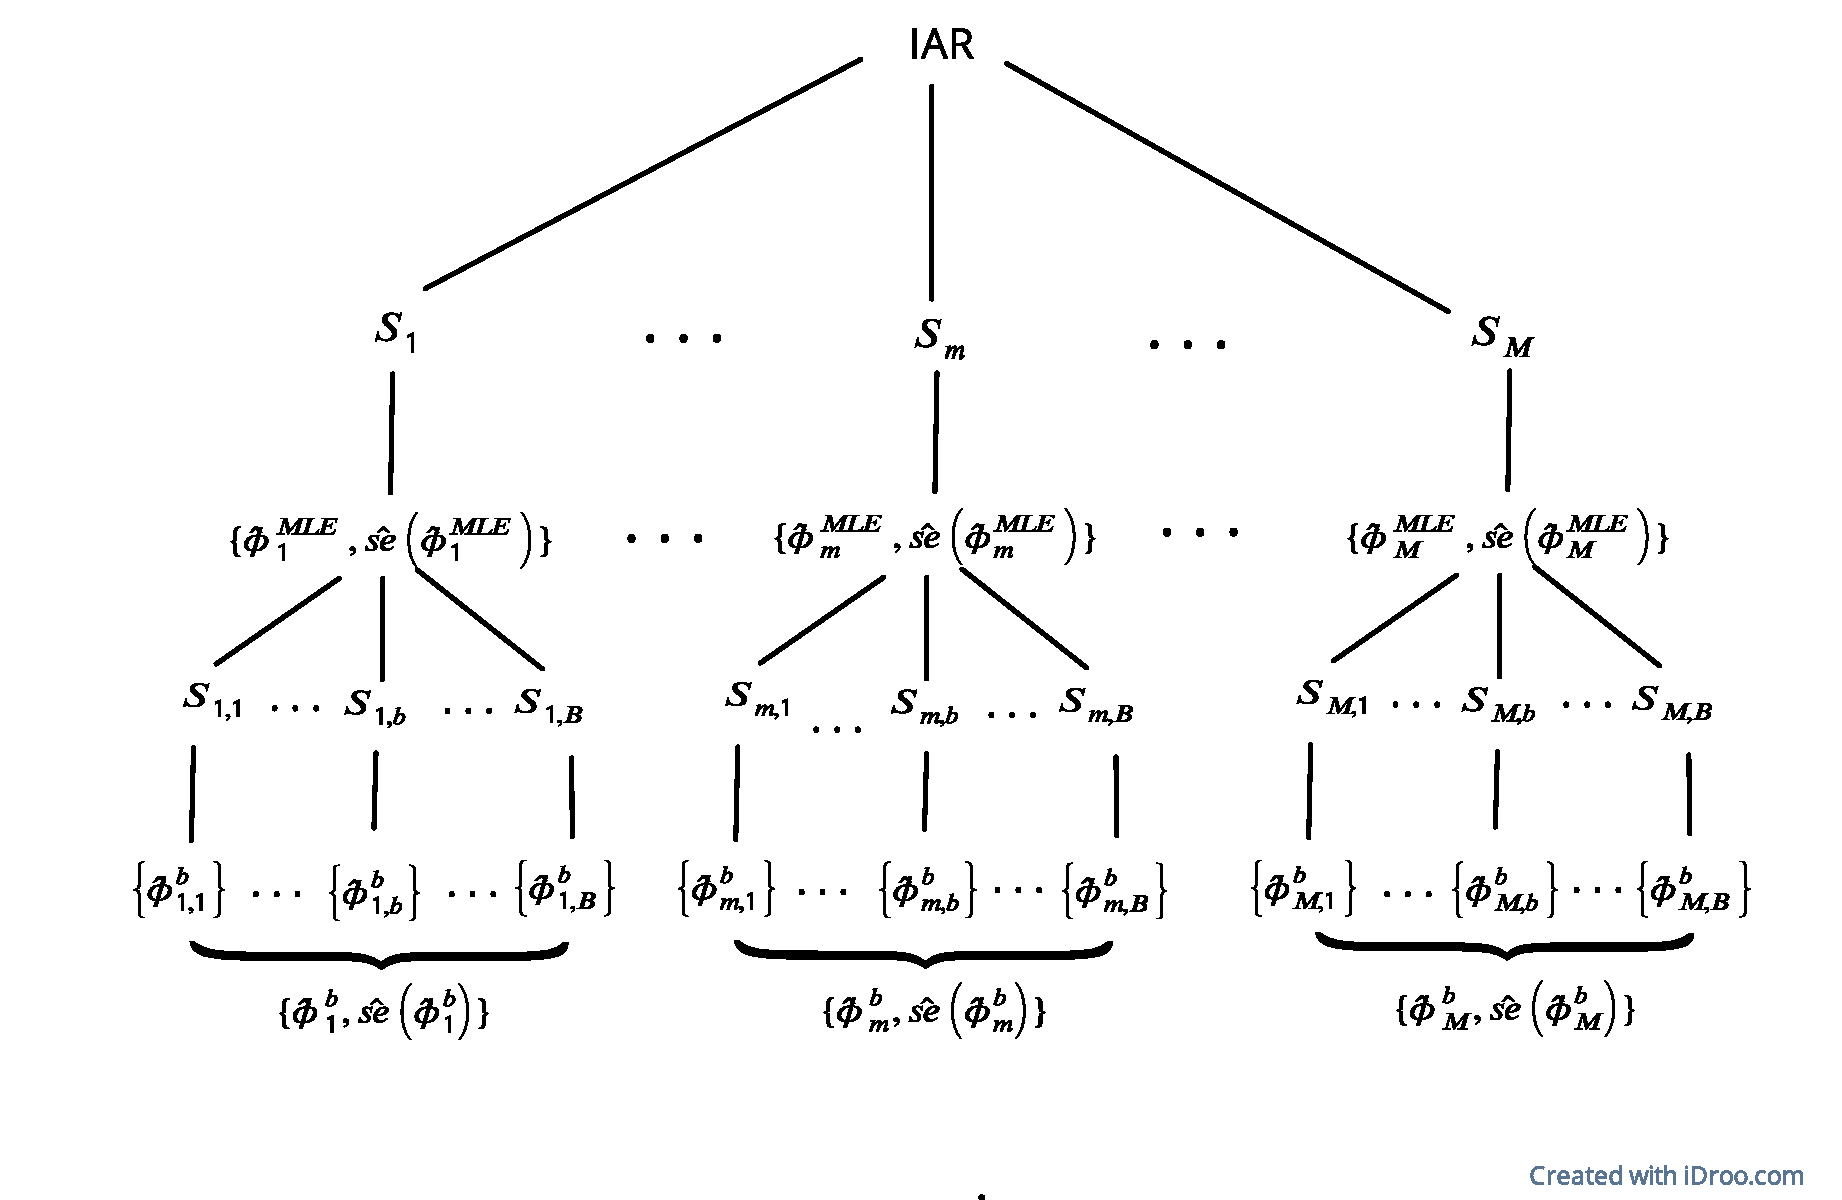
\includegraphics[trim={0 2cm 0 0},clip,width=0.9\textwidth]{Kap3/Fig_Cap3/4RzQZ8xYXY.pdf}
    \caption{Esquema general del estudio de Monte Carlo.}
    \label{fig:monte_carlo1}
\end{figure}

En este estudio, se evaluaron los resultados del modelo en el caso de tiempo irregularmente espaciado, aunque también se comprobó que el modelo es válido para tiempos regulares con $\Delta_n=1$ para todos los valores de $n$.

Para analizar el comportamiento de los estimadores de máxima verosimilitud y bootstrap, 
se realizaron simulaciones de distribuciones de muestras finitas.
Los resultados de estas simulaciones se muestran en las figuras \ref{fig:monte_carlo_res1} y \ref{fig:monte_carlo_res2}. 
Se puede observar que ambos estimadores presentan un comportamiento satisfactorio, parecen ser insesgados y consistentes en sus resultados.

Note que para valores pequeños de $n$ y para valores cercanos a cero de $\phi$, 
los estimadores tienden a tener una mayor variabilidad.
Este hallazgo es importante para el análisis de los resultados, 
ya que sugiere que la precisión de los estimadores puede verse afectada por factores como la cantidad de datos 
disponibles y la magnitud del parámetro de interés.

En segundo lugar, para ambos estimadores, presentamos las medidas de rendimiento para ambos métodos de estimación
las cuales se ven reflejadas en la tabla \ref{table:performance}

\begin{figure}[h]
    \begin{minipage}{0.45\textwidth}
    \includegraphics[width=0.8\linewidth,angle = 270]{Kap3/Fig_Cap3/sim3.eps}
    \caption{Esquema general del estudio de Monte Carlo.}
    \label{fig:monte_carlo_res1}
    \end{minipage}
    \hfill
    \begin{minipage}{0.45\textwidth}
    \includegraphics[width=0.8\linewidth,angle = 270]{Kap3/Fig_Cap3/sim4.eps}
    \caption{Esquema general del estudio de Monte Carlo.}
    \label{fig:monte_carlo_res2}
    \end{minipage}
\end{figure}

\begin{table}[h]
    \centering
    \caption{Resultados del estudio de Monte Carlo}
    \resizebox{18cm}{!} {
    \begin{tabular}{|c|cccccc|ccccc|}
    \hline
    \rowcolor[HTML]{FFFFFF} 
    \multicolumn{1}{|l|}{\cellcolor[HTML]{FFFFFF}} & \multicolumn{6}{c|}{\cellcolor[HTML]{FFFFFF}\textbf{Máxima Verosimilitud}} & \multicolumn{5}{c|}{\cellcolor[HTML]{FFFFFF}\textbf{Boostrap}} \\ \hline
    \rowcolor[HTML]{FFFFFF} 
    \multicolumn{1}{|l|}{\cellcolor[HTML]{FFFFFF}n} & \multicolumn{1}{c|}{\cellcolor[HTML]{FFFFFF}\textbf{$\phi$}} & \multicolumn{1}{c|}{\cellcolor[HTML]{FFFFFF}\textbf{$\hat{\phi}^{MLE}$}} & \multicolumn{1}{c|}{\cellcolor[HTML]{FFFFFF}\textbf{$\hat{se}(\phi^{MLE})$}} & \multicolumn{1}{c|}{\cellcolor[HTML]{FFFFFF}\textbf{$\widehat{\operatorname{bias}}_{\hat{\phi}^{MLE}}$}} & \multicolumn{1}{c|}{\cellcolor[HTML]{FFFFFF}\textbf{$\widehat{\operatorname{RMSE}}_{\hat{\phi^{MLE}}}$}} & \textbf{$\widehat{CV}_{\hat{\phi}^{MLE}}$} & \multicolumn{1}{c|}{\cellcolor[HTML]{FFFFFF}\textbf{$\hat{\phi}^{b}$}} & \multicolumn{1}{c|}{\cellcolor[HTML]{FFFFFF}\textbf{$\hat{se}(\phi^{b})$}} & \multicolumn{1}{c|}{\cellcolor[HTML]{FFFFFF}\textbf{$\widehat{\operatorname{bias}}_{\hat{\phi}^{b}}$}} & \multicolumn{1}{c|}{\cellcolor[HTML]{FFFFFF}\textbf{$\widehat{\operatorname{RMSE}}_{\hat{\phi^{b}}}$}} & \textbf{$\widehat{CV}_{\hat{\phi}^{b}}$} \\ \hline
     & \multicolumn{1}{c|}{-0.9} & \multicolumn{1}{c|}{-0.892} & \multicolumn{1}{c|}{0.029} & \multicolumn{1}{c|}{-0.008} & \multicolumn{1}{c|}{0.031} & 0.033 & \multicolumn{1}{c|}{-0.885} & \multicolumn{1}{c|}{0.032} & \multicolumn{1}{c|}{-0.015} & \multicolumn{1}{c|}{0.035} & 0.036 \\ \cline{2-12} 
     & \multicolumn{1}{c|}{-0.5} & \multicolumn{1}{c|}{-0.479} & \multicolumn{1}{c|}{0.126} & \multicolumn{1}{c|}{-0.021} & \multicolumn{1}{c|}{0.128} & 0.263 & \multicolumn{1}{c|}{-0.450} & \multicolumn{1}{c|}{0.153} & \multicolumn{1}{c|}{-0.050} & \multicolumn{1}{c|}{0.161} & 0.340 \\ \cline{2-12} 
     & \multicolumn{1}{c|}{-0.1} & \multicolumn{1}{c|}{-0.081} & \multicolumn{1}{c|}{0.210} & \multicolumn{1}{c|}{-0.019} & \multicolumn{1}{c|}{0.211} & 2.586 & \multicolumn{1}{c|}{-0.068} & \multicolumn{1}{c|}{0.222} & \multicolumn{1}{c|}{-0.032} & \multicolumn{1}{c|}{0.224} & 3.267 \\ \cline{2-12} 
     & \multicolumn{1}{c|}{0.1} & \multicolumn{1}{c|}{0.062} & \multicolumn{1}{c|}{0.211} & \multicolumn{1}{c|}{0.038} & \multicolumn{1}{c|}{0.214} & 3.388 & \multicolumn{1}{c|}{0.060} & \multicolumn{1}{c|}{0.222} & \multicolumn{1}{c|}{0.040} & \multicolumn{1}{c|}{0.226} & 3.726 \\ \cline{2-12} 
     & \multicolumn{1}{c|}{0.5} & \multicolumn{1}{c|}{0.473} & \multicolumn{1}{c|}{0.126} & \multicolumn{1}{c|}{0.027} & \multicolumn{1}{c|}{0.129} & 0.267 & \multicolumn{1}{c|}{0.450} & \multicolumn{1}{c|}{0.145} & \multicolumn{1}{c|}{0.050} & \multicolumn{1}{c|}{0.154} & 0.323 \\ \cline{2-12} 
    \multirow{-6}{*}{100} & \multicolumn{1}{c|}{0.9} & \multicolumn{1}{c|}{0.892} & \multicolumn{1}{c|}{0.029} & \multicolumn{1}{c|}{0.008} & \multicolumn{1}{c|}{0.030} & 0.033 & \multicolumn{1}{c|}{0.886} & \multicolumn{1}{c|}{0.032} & \multicolumn{1}{c|}{0.014} & \multicolumn{1}{c|}{0.035} & 0.036 \\ \hline
     & \multicolumn{1}{c|}{-0.9} & \multicolumn{1}{c|}{-0.898} & \multicolumn{1}{c|}{0.013} & \multicolumn{1}{c|}{-0.002} & \multicolumn{1}{c|}{0.013} & 0.014 & \multicolumn{1}{c|}{-0.897} & \multicolumn{1}{c|}{0.013} & \multicolumn{1}{c|}{-0.003} & \multicolumn{1}{c|}{0.013} & 0.014 \\ \cline{2-12} 
     & \multicolumn{1}{c|}{-0.5} & \multicolumn{1}{c|}{-0.495} & \multicolumn{1}{c|}{0.052} & \multicolumn{1}{c|}{-0.005} & \multicolumn{1}{c|}{0.053} & 0.106 & \multicolumn{1}{c|}{-0.491} & \multicolumn{1}{c|}{0.054} & \multicolumn{1}{c|}{-0.009} & \multicolumn{1}{c|}{0.055} & 0.110 \\ \cline{2-12} 
     & \multicolumn{1}{c|}{-0.1} & \multicolumn{1}{c|}{-0.101} & \multicolumn{1}{c|}{0.110} & \multicolumn{1}{c|}{0.001} & \multicolumn{1}{c|}{0.110} & 1.095 & \multicolumn{1}{c|}{-0.097} & \multicolumn{1}{c|}{0.111} & \multicolumn{1}{c|}{-0.003} & \multicolumn{1}{c|}{0.111} & 1.153 \\ \cline{2-12} 
     & \multicolumn{1}{c|}{0.1} & \multicolumn{1}{c|}{0.091} & \multicolumn{1}{c|}{0.111} & \multicolumn{1}{c|}{0.009} & \multicolumn{1}{c|}{0.112} & 1.227 & \multicolumn{1}{c|}{0.087} & \multicolumn{1}{c|}{0.111} & \multicolumn{1}{c|}{0.013} & \multicolumn{1}{c|}{0.112} & 1.274 \\ \cline{2-12} 
     & \multicolumn{1}{c|}{0.5} & \multicolumn{1}{c|}{0.495} & \multicolumn{1}{c|}{0.052} & \multicolumn{1}{c|}{0.005} & \multicolumn{1}{c|}{0.052} & 0.105 & \multicolumn{1}{c|}{0.491} & \multicolumn{1}{c|}{0.054} & \multicolumn{1}{c|}{0.009} & \multicolumn{1}{c|}{0.054} & 0.109 \\ \cline{2-12} 
    \multirow{-6}{*}{500} & \multicolumn{1}{c|}{0.9} & \multicolumn{1}{c|}{0.899} & \multicolumn{1}{c|}{0.013} & \multicolumn{1}{c|}{0.001} & \multicolumn{1}{c|}{0.013} & 0.014 & \multicolumn{1}{c|}{0.898} & \multicolumn{1}{c|}{0.013} & \multicolumn{1}{c|}{0.002} & \multicolumn{1}{c|}{0.013} & 0.014 \\ \hline
     & \multicolumn{1}{c|}{-0.9} & \multicolumn{1}{c|}{-0.900} & \multicolumn{1}{c|}{0.007} & \multicolumn{1}{c|}{0.000} & \multicolumn{1}{c|}{0.007} & 0.008 & \multicolumn{1}{c|}{-0.899} & \multicolumn{1}{c|}{0.007} & \multicolumn{1}{c|}{-0.001} & \multicolumn{1}{c|}{0.007} & 0.008 \\ \cline{2-12} 
     & \multicolumn{1}{c|}{-0.5} & \multicolumn{1}{c|}{-0.498} & \multicolumn{1}{c|}{0.030} & \multicolumn{1}{c|}{-0.002} & \multicolumn{1}{c|}{0.030} & 0.060 & \multicolumn{1}{c|}{-0.497} & \multicolumn{1}{c|}{0.030} & \multicolumn{1}{c|}{-0.003} & \multicolumn{1}{c|}{0.030} & 0.060 \\ \cline{2-12} 
     & \multicolumn{1}{c|}{-0.1} & \multicolumn{1}{c|}{-0.098} & \multicolumn{1}{c|}{0.066} & \multicolumn{1}{c|}{-0.002} & \multicolumn{1}{c|}{0.066} & 0.673 & \multicolumn{1}{c|}{-0.096} & \multicolumn{1}{c|}{0.066} & \multicolumn{1}{c|}{-0.004} & \multicolumn{1}{c|}{0.066} & 0.688 \\ \cline{2-12} 
     & \multicolumn{1}{c|}{0.1} & \multicolumn{1}{c|}{0.096} & \multicolumn{1}{c|}{0.067} & \multicolumn{1}{c|}{0.004} & \multicolumn{1}{c|}{0.067} & 0.695 & \multicolumn{1}{c|}{0.094} & \multicolumn{1}{c|}{0.066} & \multicolumn{1}{c|}{0.006} & \multicolumn{1}{c|}{0.067} & 0.705 \\ \cline{2-12} 
     & \multicolumn{1}{c|}{0.5} & \multicolumn{1}{c|}{0.500} & \multicolumn{1}{c|}{0.030} & \multicolumn{1}{c|}{0.000} & \multicolumn{1}{c|}{0.030} & 0.059 & \multicolumn{1}{c|}{0.498} & \multicolumn{1}{c|}{0.030} & \multicolumn{1}{c|}{0.002} & \multicolumn{1}{c|}{0.030} & 0.060 \\ \cline{2-12} 
    \multirow{-6}{*}{1500} & \multicolumn{1}{c|}{0.9} & \multicolumn{1}{c|}{0.900} & \multicolumn{1}{c|}{0.007} & \multicolumn{1}{c|}{0.000} & \multicolumn{1}{c|}{0.007} & 0.008 & \multicolumn{1}{c|}{0.899} & \multicolumn{1}{c|}{0.007} & \multicolumn{1}{c|}{0.001} & \multicolumn{1}{c|}{0.007} & 0.008 \\ \hline
    \end{tabular}
    }
    \label{table:performance}
    \end{table}

\clearpage
\newpage

\section{Comparación del Modelo IAR vs el CIAR}
En este apartado, nos disponemos a comparar nuestra solución, con la solucion propuesta en \cite{elorrieta2019discrete}
descrita en la sección \ref{section:CIAR} (El modelo CIAR), para ello, se plantea un escenario de simulación similar al de la sección anterior, donde,
$\sigma_0 = 1$, $\phi_0 \in \lbrace -0.1 , -0.5, -0.9\rbrace$, $n \in \lbrace100, 5000, 1500\rbrace$ y $\Delta_n = \tau_n - \tau_{n-1} \sim 1 + poisson(\lambda = 2)$. En este caso solo simulamos muestras aleatorias con parametro negativo ya que es el foco de este estudio. En el caso del IAR, se asumen que 
$\phi^{I} = 0$ (la parte imaginaria es cero) y que $c = 0$. Para comparar nuestro modelo con el CIAR, utilizaremos el \emph{Error cuadrático medio (ECM)}, que definiremos así

$$ECM = \sqrt{\frac{\sum_{i=1}^{n}(e_i - \bar{e})^2}{n}}$$

donde $e_i = X_{t_i} - \hat{X}_{\tau_i}$ para $i = 1, ..., n$.
\begin{figure}[h]
    \begin{minipage}{0.45\textwidth}
    \includegraphics[width=0.75\linewidth,angle = 270]{Kap3/Fig_Cap3/sim4_IARvsCIAR.eps}
    \caption{Comportamiento de la simulación, tomando como base el IAR.}
    \label{fig:iarvsciar}
    \end{minipage}
    \hfill
    \begin{minipage}{0.45\textwidth}
    \includegraphics[width=0.75\linewidth,angle = 270]{Kap3/Fig_Cap3/sim4_CIARvsIAR.eps}
    \caption{Comportamiento de la simulación, tomando como base el CIAR.}
    \label{fig:ciarvsiar}
    \end{minipage}
\end{figure}

la figura \ref{fig:iarvsciar} muestra el resultado de la simulacion de un IAR con las condiciones dadas, y estimando tanto  el IAR como el CIAR
con los mismos datos simulados y midiendo el ECM de la predicción. Por otra parte la figura \ref{fig:ciarvsiar} muestra los mismos resultados pero esta vez,
los datos fueron simulados a partir del CIAR.

Esta simulacion permite llevarnos a la conclusión de que, cuando el parámetro $\phi_n \to -1$ el modelo IAR tiene un rendimiento mucho mejor en cuanto al ECM. 
Por otra parte cuando el parámetro $\phi \to 0$ el CIAR presenta un mejor comportamiento, sobre todo en muestras grandes. Y cuando $phi$ esta al rededor de 0.5, el CIAR muestra
un mejor rendimiento en muestras pequeñas, pero el IAR es mejor para muestras grandes, este comportamiento es identico tanto simulando IAR como CIAR.


\section{Aplicación en datos de espeleotemas\protect\footnote{Los espeleotemas son formaciones geológicas que se encuentran en cuevas y se forman a partir de la acumulación de minerales depositados por el agua que gotea del techo o fluye por las paredes de la cueva. Algunos ejemplos de espeleotemas incluyen estalactitas, estalagmitas, columnas y cortinas de piedra caliza.}}

Estos datos han sido descritos y trabajados por \cite{mudelse2014climate} en su libro y los hemos encontrado disponibles en la \href{https://www.manfredmudelsee.com/}{pagina web del autor}. Este conjunto de datos cuenta con 1345 datos donde se miden el pocentaje de 
isotopos de oxigeno 18 y 16 estables; $\delta^{18}O$ a travez de los años, la escala de tiempo (para años antes de 1950) es basada en
se basada en 18 edades espectrométricas de masa $U/Th$. La figura \ref{fig:example} muestra el comportamiento de la serie de tiempo descrita y la figura 
\ref{fig:example_delta} muestra el comportamiento irregularmente espaciado entre los tiempos, note que si esta fuera una serie regular, este grafico seríá una
linea constante horizontal en $y=1$



\begin{figure}[h]
    \begin{minipage}{0.45\textwidth}
    \includegraphics[width=0.8\linewidth,angle = 270]{Kap3/Fig_Cap3/example_data_original.eps}
    \caption{Comportamiento de la serie de tiempo.}
    \label{fig:example}
    \end{minipage}
    \hfill
    \begin{minipage}{0.45\textwidth}
    \includegraphics[width=0.8\linewidth,angle = 270]{Kap3/Fig_Cap3/example_delta.eps}
    \caption{Comportamiento del $\Delta_n$ de la serie.}
    \label{fig:example_delta}
    \end{minipage}
\end{figure}

Ahora procedemos a realizar nuestras estimaciones tanto por Bootstrap como por Máxima Verosimilitud, en este caso, ejemplificamos el uso tanto en la serie original
como en la serie diferenciada, esta diferenciacion se realiza con el fin de eliminar tendencias y comportamientos ciclicos en nuestra serie
de tiempo, este caso, $\nabla X_{\tau_n} = X_{\tau_n}-X_{\tau_{n-1}}$ es la serie diferenciada. La figure \ref{fig:example_diff_fit}
muestra el resultado de la serie diferenciada y la figura \ref{fig:example_fit} muestra los resultados para la serie original.

Los parametros estimados para la serie original son los siguientes:

$$\hat{\phi}^{MLE}= 0.997 \quad \hat{se}(\phi^{MLE})=0.0007 \quad \hat{\sigma}^{2}_{MLE}=0.0112 \quad \hat{se}(\hat{\sigma}^{2}_{MLE})=0.0020$$
$$\hat{\phi}^{b}= 0.997 \quad \hat{se}(\phi^{b})=0.00086 \quad \hat{\sigma}^{2}_{b}=0.0069  \quad \hat{se}(\hat{\sigma}^{2}_{b})=0.0020$$

Seguido a esto, calculamos los parametros para la serie diferenciada obteniendo:
$$\hat{\phi}^{MLE}= -0.790 \quad \hat{se}(\phi^{MLE})=0.0136 \quad \hat{\sigma}^{2}_{MLE}=0.0190 \quad \hat{se}(\hat{\sigma}^{2}_{MLE})=0.0037$$
$$\hat{\phi}^{b}= -0.789 \quad \hat{se}(\phi^{b})=0.0149 \quad \hat{\sigma}^{2}_{b}= 0.0167  \quad \hat{se}(\hat{\sigma}^{2}_{b})=0.04785$$


\begin{figure}[h]
    \begin{minipage}{0.45\textwidth}
    \includegraphics[width=0.8\linewidth,angle = 270]{Kap3/Fig_Cap3/example_data_original_estimation.eps}
    \caption{Comportamiento del modelo estimado con la serie original.}
    \label{fig:example_fit}
    \end{minipage}
    \hfill
    \begin{minipage}{0.45\textwidth}
    \includegraphics[width=0.8\linewidth,angle = 270]{Kap3/Fig_Cap3/example_data_diff_estimation.eps}
    \caption{Comportamiento del modelo estimado con la serie diferenciada.}
    \label{fig:example_diff_fit}
    \end{minipage}
\end{figure}



